\section{Исследовательская часть}
\subsection{Постановка задачи на исследование}
Для детального изучения поведения метода при разных условиях проводится несколько исследований.

Необходимо рассмотреть, как размер выборки влияет на меру сходства.

Следует также проанализировать, как влияет размер выборки на качество определения объекта по косинусному сходству: какова доля обращений к вспомогательному методу, основанному на сети синтаксических графов, а также какой процент этих обращений приходится на неверное предположение.

При обращении к дополняющему методу необходимая сеть создаётся <<на лету>> на основе терминов, которые были отобраны на предыдущем шаге с применением косинусного расстояния. Следует оценить, как отличается время выполнения при таком подходе по сравнению с использованием заранее сформированной сети по всей онтологии. \newline

\textbf{Характеристики компьютера}

Все проведённые эксперименты проводились на персональном компьютере с характеристиками:
\begin{itemize}
	\item операционная система --- Windows 10, 64-разрядная;
	\item процессор --- Intel(R) Core(TM) i7-10510U CPU @ 1.80GHz 2.30 GHz;
	\item оперативная память --- 16,00 ГБ. \\
\end{itemize}

\subsection{Проведение исследований}

\subsubsection{Влияние размера выборки на меру сходства}
Для проведения эксперимента использовались онтологии \, следующих \, размеров: 100, 250, 450, 600. В качестве входных данных выступают определения из предметного словаря.  Исследование построено на предположении, что малый размер датасета не позволяет в достаточной степени определить сходство двух определений.

Результаты исследования были сведены в таблицу \ref{table_research}.

\begin{longtable}{|p{5cm}|p{1.5cm}|p{1.5cm}|p{1.5cm}|p{1.5cm}|p{1.5cm}|}
	\caption{Влияние размера выборки на меру сходства}\label{table_research}\\
	\hline
	
	\textbf{Термины} & \multicolumn{5}{|c|}{\textbf{Размер выборки}}\\ 
	\cline{2-6}
	& \textbf{100} & \textbf{250} & \textbf{300} & \textbf{450} & \textbf{600} \\
	\hline
	\endfirsthead
	
	\hline
	\textbf{Термины} & \multicolumn{5}{|c|}{\textbf{Размер выборки}}\\ 
	\cline{2-6}
	& \textbf{100} & \textbf{250} & \textbf{300} & \textbf{450} & \textbf{600} \\
	\hline
	\endhead
	
	\hline
	\multicolumn{6}{c}{\textit{Продолжение на следующей странице}}
	\endfoot
	\hline
	\endlastfoot
	
	аккумуляторный элемент & 0.066 & 0.092 & 0.149 & 0.267 & 0.358\\
	\hline
	блокировка пуска & 0.135 & 0.099 & 0.138 & 0.384 & 0.566\\
	\hline
	гистерезис регyлятора & 0.113 & 0.105 & 0.110 & 0.121 & 0.152 \\
	\hline
	глушитель шума & 0.198 & 0.566 & 0.661 & 0.615 & 0.686\\ 
	\hline
	двигатель внутреннего сгорания & 0.107 & 0.051 & 0.191 & 0.227 & 0.268 \\ 
	\hline
	дефлектор & 0.316 & 0.447 & 0.519 & 0.504 & 0.535\\ 
	\hline
	зубчатый ремень & 0.0 & 0.159 & 0.194 & 0.286 & 0.347\\ 
	\hline
	изотермический процесс & 0.408 & 0.615 & 0.815 & 0.97 & 0.991\\
	\hline
	изохорный процесс & 0.671 & 0.811 & 0.949 & 0.975 & 0.984\\
	\hline
	рабочее тело & 0.0 & 0.0 & 0.221 & 0.282 & 0.33 
\end{longtable}

Исходя из приведённой выше таблицы можно сделать следующие выводы.
\begin{itemize}
	\item Как правило, с увеличением размера выборки увеличивается и мера сходства между определением из онтологии и соответствующим запросом, имеет место накопительный характер формирования базы знаний, что \, можно увидеть на примере терминов <<аккумуляторный элемент>>, <<глушитель шума>>. 
	
	\item Случаи, когда накопление данных приводит к обратному \, результату: \, уменьшение меры, объясняются человеческим фактором. Каждый \, из \, опрашиваемых давал определение в той формулировке, которая казалась ему наиболее понятной и правильной, таким образом, термины описывались с разных сторон. Примером может послужить <<блокировка пуска>>.
	
	\item Также в онтологии есть термины, которые вызвали большое затруднение у опрашиваемых, среди них <<гистерезис регулятора>>. Многие студенты не знали, что это такое, либо ошибались в своих предположениях, поэтому косинусная мера сходства с увеличением выборки росла незначительно.
	
	\item Кроме того, существуют многозначные, сложные термины (например, \, <<двигатель внутреннего сгорания>>). В силу этого выявить схожие формулировки, ключевые слова довольно сложно. Определение из онтологии таких терминов, как правило, содержит много слов с малым весом, что определяет малую меру сходства с запросом пользователя.
	
	\item При вычислении косинусного сходства между определением из онтологии и запросом пользователя возможен случай, когда мера сходства равна 0. Это означает, что у рассматриваемой пары определений нет ничего общего. Такая ситуация возможна в двух случаях: когда сравниваются определения разных, непохожих терминов и когда онтология не достаточно полная и качественная. Похожую ситуация можно наблюдать с терминами <<зубчатый ремень>> и <<рабочее тело>>. 
	
	\item Существует ряд терминов, формулировки определений которых \, однозначны, известны большинству. В таком случае, мера сходства даже при маленьком объёме онтологии будет принимать существенно \, бо́льшее \, значение, нежели остальные термины, которые были описаны выше. А с увеличением выборки всё больше будет расти. В качестве примера можно привести <<изотермический процесс>> и <<изохорный процесс>>. \\
\end{itemize}

\subsubsection{Влияние размера выборки на процент обращения к вспомогательному методу}
Исследование проводилось на датасетах размерами 100, 150, 250, 400 и 650 определений. 

Для всех наборов данных вычислялись ключевые слова и их вес в рамках рассматриваемой онтологии для каждого из 50 терминов. Затем проверялись определения из предметного словаря на каждой из созданной онтологии. 

Каждый раз, когда результат применения статистического метода оценки не проходит по критерию принятия решения, фиксируется обращение к дополняющему методу. Для получения статистики по неверным результатам, полученный ответ сравнивается с правильным.

В итоге, по полученным значениям строится диаграмма, представленная на рисунке \ref{fig400:image}.

\begin{figure}[h!]
	\begin{center}
		{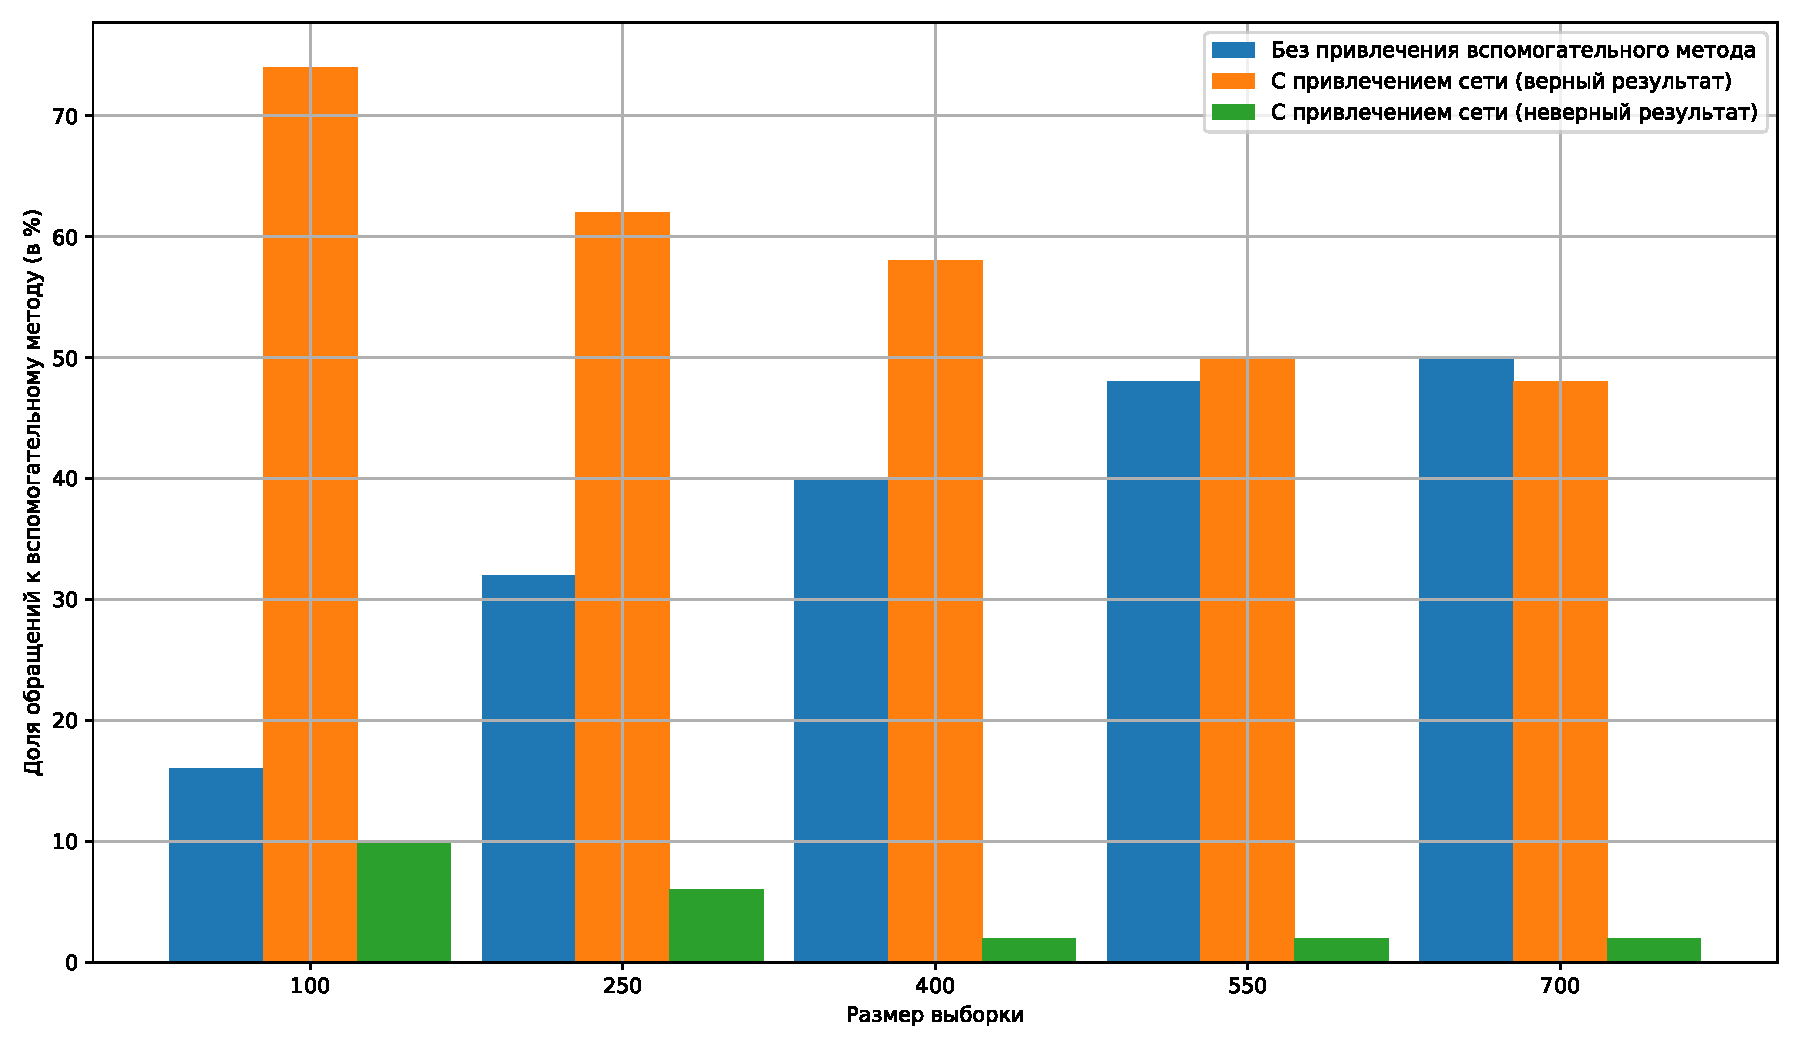
\includegraphics[scale = 0.54]{img/research/time3.pdf}}
		\caption{Влияние размера выборки на процент обращения к вспомогательному методу.}
		\label{fig400:image}
	\end{center}
\end{figure}

По диаграмме можно сделать следующие выводы.
\begin{itemize}
	\item На маленьком датасете (100 определений) доля обращений к дополняющему методу очень высока (более 80\%), из них 10\% приходится на неверный результат.
	
	\item В целом, с увеличением размера данных корректность работы статистического метода увеличивается, о чём свидетельствует увеличивающийся процент. Так, доля запросов, которые обрабатываются без привлечения вспомогательного метода при объёме данных в 700 определений больше примерно на 34\%, чем при 100 элементах, что потенциально сокращает время обработки запроса пользователя.
	
	\item Аналогичная ситуация наблюдается с процентом неправильных ответов, которые даются при обработке вспомогательным методом, он также снижается. Это обуславливается, прежде всего, тем, что алгоритм косинусного сходства с увеличением выборки лучше идентифицирует потенциально верные термины, из которых на втором этапе алгоритма строится сеть. \newline
\end{itemize}

\subsubsection{Сравнение времени поиска по частичной и полной сети}
В качестве входных данных также используются определения из предметного словаря, и только те, где результат применения косинусного сходства не удовлетворяет критерию принятия решений. 

Исследование проводится на онтологии максимального размера (около 800 определений).

Для сопоставления \, времени \, выполнения \, используется библиотека \, time \cite{time}. 

Количество узлов в сети, которая создаётся <<на лету>>, определяется результатом статистического метода. Полная сеть включает в себя все термины онтологии, формируется заранее и только один раз, а затем хранится в сопутствующей базе данных, откуда извлекается для проведения этого исследования. В отличие от подхода с использованием полной сети, в частичной сети помимо поиска ещё необходимо учитывать время на формирование этой сети. 

В результате была получена диаграмма, изображённая на рисунке \ref{fig403:image}.
\begin{figure}[h!]
	\begin{center}
		{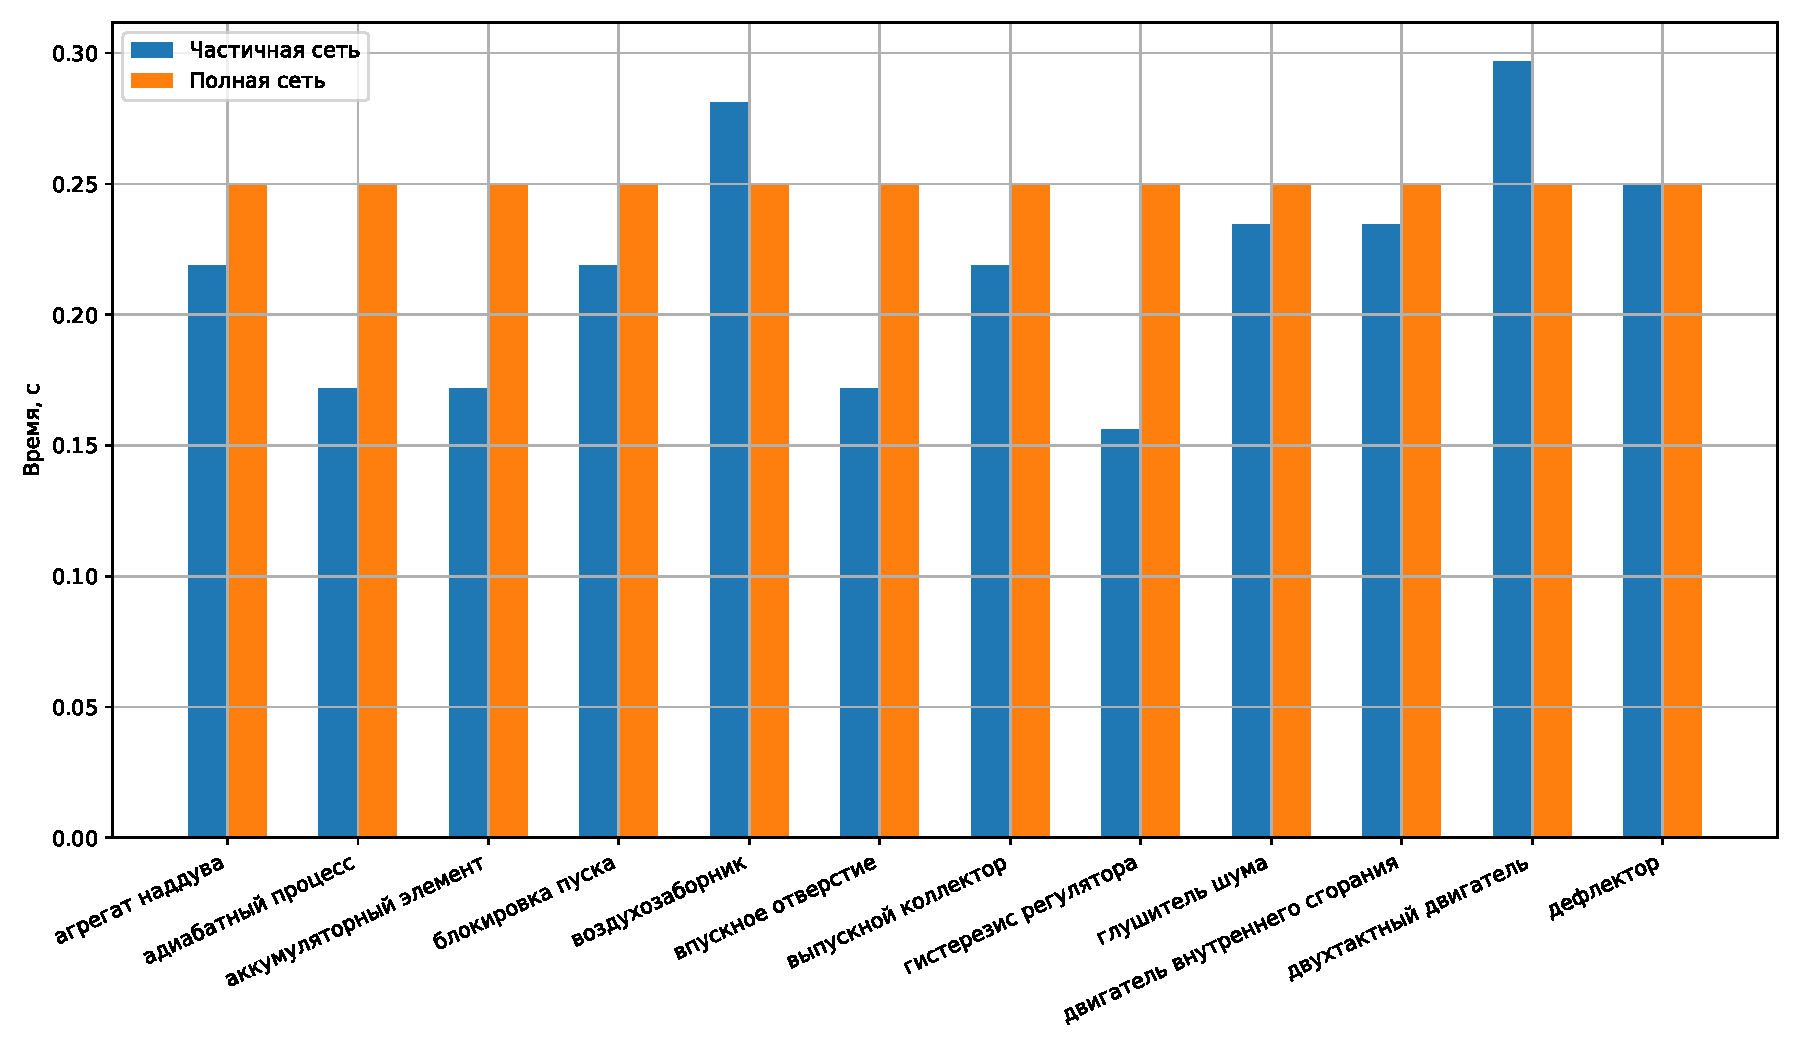
\includegraphics[scale = 0.54]{img/research/time.pdf}}
		\caption{Сравнение времени поиска по частичной и полной сети.}
		\label{fig403:image}
	\end{center}
\end{figure}

По диаграмме можно сделать следующие выводы.
\begin{itemize}
	\item Как правило, подход с использованием частичной сети затрачивает меньше времени, несмотря на то, что дополнительно осуществляется формирование сети.
	
	\item В силу того, что полная сеть постоянна от запроса к запросу, то время обработки ожидаемо одинаковое на всех терминах.
	
	\item Несмотря на то, что в большинстве случаев неполная сеть быстрее обрабатывает запрос, иногда наблюдается обратная динамика, например, это касается терминов <<воздухозаборник>>, <<двухтактный двигатель>>. Объяснятся тем, что помимо поиска учитывается формирование сети. Соответственно, чем больше потенциально верных терминов было отобрано на этапе определений косинусных сходств, тем больше времени потребуется сети для ответа на запрос. \\
\end{itemize}
 
\subsection*{Выводы}
%\addcontentsline{toc}{subsection}{Выводы}
Было проведено несколько исследований на предмет изучения поведения разработанного метода при разных условиях.
Было проведено несколько испытаний на предмет того:
\begin{itemize}
	\item как размер выборки влияет в общем на меру сходства между определением из онтологии и запросом пользователя;
	
	\item как размер выборки оказывает влияние на процент обращения к вспомогательному методу;
	
	\item стоит ли использовать частичную сеть, которая строится по ходу выполнения программы, когда можно использовать заранее подготовленную по всей онтологии сеть. \\
\end{itemize}
%
В результате всех указанных исследований можно сделать общий вывод.
\begin{itemize}
	\item Если привлекать качественную выборку (т.е. включающую в основном правильные, полные определения), то с увеличением выборки, растёт и мера сходства.
	
	\item Также с увеличением выборки, уменьшается доля обращений к вспомогательному методу на основе сети, что позволяет сократить время обработки запроса. Кроме того, сокращается и число случаев, когда сеть определяет термин неверно.
	
	\item Несмотря на то, что тратится дополнительно время на формирование частичной сети, такой подход всё равно обрабатывает запрос быстрее, чем это делается в полной сети, построенной заранее.
\end{itemize}